\section{Additional results}
\label{app:additional}

\subsection{The 300B factorial in full}
\label{app:factorial}

Table~\ref{tab:factorial_perbenchmark} gives the per-benchmark values behind
Section~\ref{sec:factorial} for all thirty-six evaluated checkpoints, and
Table~\ref{tab:factorial_language} gives the language-understanding suite for the twelve
distinct pre-training runs. Two patterns in the language table are worth naming. Without
front-loading, FineWeb-Edu and the permissive substrate score at chance on both 5-shot
MMLU and 10-shot CommonsenseQA, and front-loading moves them well above it, so part of
what instruction and reasoning data supplies is the ability to answer a benchmark in the
format it asks for. Nemotron-CC-HQ is the exception, retaining $46.4$ on MMLU and $48.6$
on CommonsenseQA without front-loading, which is consistent with its construction from
classifier-filtered and synthetically rephrased web text and explains why it gains least
from the subset.

Figure~\ref{fig:fl_trajectory} shows how the front-loading effect evolves across
post-training stages. It is largest at the base stage and shrinks under Phase 1 without
disappearing, which is the same statement as the observation in Section~\ref{sec:factorial}
that Tulu3 recovers only part of the deficit created by omitting the subset.
Figure~\ref{fig:domains} decomposes the effect by capability domain. Table~\ref{tab:phase1_zoo_full} gives both context variants for every model in the zoo, of which Table~\ref{tab:phase1_zoo} in the main text shows one per family.

% Generated by generate_workshop_artifacts.py. Do not edit by hand.
\begin{table}[t]
\centering
\caption{Phase~1 (Tulu3 SFT and DPO) across the model zoo at 1.7B scale, both context variants. This is the complete version of Table~\ref{tab:phase1_zoo}. Protocol~A (Appendix Table~\ref{tab:eval-settings-A}). Values are mean$_{\pm\text{SD}}$ over decoding seeds 42, 1234, and 2025.}
\label{tab:phase1_zoo_full}
\scriptsize
\setlength{\tabcolsep}{3pt}
\resizebox{\linewidth}{!}{%
\begin{tabular}{lrrrrrrrrrrrr}
\toprule
\textbf{Model} & \textbf{A24} & \textbf{A25} & \textbf{AMC} & \textbf{M500} & \textbf{GSM8K} & \textbf{HE} & \textbf{LCB} & \textbf{MBPP} & \textbf{GPQA} & \textbf{JEE} & \textbf{IFE} & \textbf{Avg} \\
\midrule
\addlinespace[0.15em]
\multicolumn{13}{l}{\textit{Matched compute, 300B tokens, controlled comparison}} \\
\addlinespace[0.2em]
MixtureVitae & 0.0$_{\pm0.00}$ & 7.8$_{\pm5.09}$ & 5.0$_{\pm0.00}$ & 17.8$_{\pm0.72}$ & 54.1$_{\pm0.00}$ & 13.6$_{\pm0.93}$ & 13.1$_{\pm1.36}$ & 19.5$_{\pm0.12}$ & 24.4$_{\pm0.77}$ & 2.9$_{\pm0.51}$ & 36.2$_{\pm0.13}$ & 17.7$_{\pm0.29}$ \\
\quad $\to$ SFT & 0.0$_{\pm0.00}$ & 0.0$_{\pm0.00}$ & 12.5$_{\pm0.00}$ & 29.5$_{\pm0.23}$ & 49.9$_{\pm0.00}$ & 44.3$_{\pm0.70}$ & 2.4$_{\pm0.11}$ & 39.9$_{\pm0.23}$ & 20.7$_{\pm0.87}$ & 3.7$_{\pm0.55}$ & 49.8$_{\pm0.13}$ & 23.0$_{\pm0.16}$ \\
\quad $\to$ SFT $\to$ DPO & 0.0$_{\pm0.00}$ & 3.3$_{\pm0.00}$ & 10.8$_{\pm1.44}$ & 30.5$_{\pm0.12}$ & 50.2$_{\pm0.00}$ & 47.4$_{\pm0.35}$ & 2.0$_{\pm0.20}$ & 41.2$_{\pm0.20}$ & 21.2$_{\pm0.00}$ & 4.5$_{\pm0.34}$ & 52.2$_{\pm0.20}$ & 23.9$_{\pm0.17}$ \\
\midrule
\addlinespace[0.2em]
MixtureVitae-16K & 1.1$_{\pm1.92}$ & 3.3$_{\pm0.00}$ & 23.3$_{\pm8.04}$ & 47.0$_{\pm0.53}$ & 60.0$_{\pm0.00}$ & 54.1$_{\pm0.35}$ & 22.3$_{\pm0.34}$ & 40.1$_{\pm0.23}$ & 23.4$_{\pm0.29}$ & 8.0$_{\pm0.24}$ & 54.6$_{\pm0.23}$ & 30.7$_{\pm0.72}$ \\
\quad $\to$ SFT & 3.3$_{\pm0.00}$ & 3.3$_{\pm0.00}$ & 15.0$_{\pm0.00}$ & 35.0$_{\pm0.53}$ & 51.6$_{\pm0.00}$ & 54.1$_{\pm0.35}$ & 14.4$_{\pm0.11}$ & 40.4$_{\pm0.35}$ & 23.4$_{\pm0.29}$ & 5.1$_{\pm0.27}$ & 55.1$_{\pm0.26}$ & 27.3$_{\pm0.11}$ \\
\quad $\to$ SFT $\to$ DPO & 3.3$_{\pm0.00}$ & 1.1$_{\pm1.92}$ & 17.5$_{\pm0.00}$ & 37.0$_{\pm0.80}$ & 52.6$_{\pm0.00}$ & 52.6$_{\pm0.70}$ & 14.6$_{\pm0.30}$ & 40.3$_{\pm0.12}$ & 23.4$_{\pm0.29}$ & 6.2$_{\pm0.20}$ & 56.5$_{\pm0.74}$ & 27.8$_{\pm0.04}$ \\
\midrule
\addlinespace[0.2em]
Nemotron-CC-HQ & 0.0$_{\pm0.00}$ & 0.0$_{\pm0.00}$ & 0.0$_{\pm0.00}$ & 0.2$_{\pm0.00}$ & 4.1$_{\pm0.00}$ & 0.0$_{\pm0.00}$ & 0.0$_{\pm0.00}$ & 2.4$_{\pm0.00}$ & 5.7$_{\pm0.29}$ & 0.0$_{\pm0.00}$ & 30.3$_{\pm0.20}$ & 3.9$_{\pm0.01}$ \\
\quad $\to$ SFT & 0.0$_{\pm0.00}$ & 0.0$_{\pm0.00}$ & 5.0$_{\pm0.00}$ & 3.1$_{\pm0.23}$ & 6.8$_{\pm0.00}$ & 4.9$_{\pm0.00}$ & 0.2$_{\pm0.00}$ & 5.5$_{\pm0.23}$ & 20.2$_{\pm0.00}$ & 2.0$_{\pm0.17}$ & 40.5$_{\pm0.27}$ & 8.0$_{\pm0.04}$ \\
\quad $\to$ SFT $\to$ DPO & 0.0$_{\pm0.00}$ & 0.0$_{\pm0.00}$ & 2.5$_{\pm0.00}$ & 3.5$_{\pm0.42}$ & 8.0$_{\pm0.00}$ & 6.1$_{\pm0.00}$ & 0.2$_{\pm0.00}$ & 5.1$_{\pm0.12}$ & 21.2$_{\pm0.00}$ & 2.7$_{\pm0.66}$ & 42.1$_{\pm0.39}$ & 8.3$_{\pm0.07}$ \\
\midrule
\addlinespace[0.2em]
Nemotron-CC-HQ-16K & 0.0$_{\pm0.00}$ & 0.0$_{\pm0.00}$ & 0.0$_{\pm0.00}$ & 2.8$_{\pm0.35}$ & 8.2$_{\pm0.00}$ & 1.8$_{\pm0.00}$ & 0.1$_{\pm0.11}$ & 5.7$_{\pm0.31}$ & 22.7$_{\pm0.51}$ & 5.6$_{\pm1.04}$ & 42.7$_{\pm0.38}$ & 8.1$_{\pm0.08}$ \\
\quad $\to$ SFT & 0.0$_{\pm0.00}$ & 0.0$_{\pm0.00}$ & 0.0$_{\pm0.00}$ & 2.9$_{\pm0.31}$ & 8.6$_{\pm0.00}$ & 5.3$_{\pm0.35}$ & 0.0$_{\pm0.00}$ & 5.9$_{\pm0.12}$ & 22.2$_{\pm0.87}$ & 1.2$_{\pm0.08}$ & 45.8$_{\pm0.00}$ & 8.4$_{\pm0.12}$ \\
\quad $\to$ SFT $\to$ DPO & 0.0$_{\pm0.00}$ & 0.0$_{\pm0.00}$ & 2.5$_{\pm0.00}$ & 2.5$_{\pm0.12}$ & 7.7$_{\pm0.00}$ & 5.3$_{\pm0.35}$ & 0.0$_{\pm0.00}$ & 5.3$_{\pm0.12}$ & 23.4$_{\pm1.17}$ & 1.7$_{\pm0.37}$ & 46.3$_{\pm0.61}$ & 8.6$_{\pm0.06}$ \\
\midrule
\addlinespace[0.2em]
FineWeb-Edu & 0.0$_{\pm0.00}$ & 0.0$_{\pm0.00}$ & 0.0$_{\pm0.00}$ & 0.0$_{\pm0.00}$ & 3.2$_{\pm0.00}$ & 0.0$_{\pm0.00}$ & 0.0$_{\pm0.00}$ & 0.0$_{\pm0.00}$ & 25.1$_{\pm0.58}$ & 0.0$_{\pm0.00}$ & 38.1$_{\pm0.08}$ & 6.0$_{\pm0.06}$ \\
\quad $\to$ SFT & 0.0$_{\pm0.00}$ & 0.0$_{\pm0.00}$ & 0.0$_{\pm0.00}$ & 2.1$_{\pm0.12}$ & 7.1$_{\pm0.00}$ & 2.4$_{\pm0.00}$ & 0.0$_{\pm0.00}$ & 2.3$_{\pm0.23}$ & 26.9$_{\pm0.58}$ & 1.6$_{\pm0.46}$ & 35.3$_{\pm0.15}$ & 7.1$_{\pm0.07}$ \\
\quad $\to$ SFT $\to$ DPO & 0.0$_{\pm0.00}$ & 0.0$_{\pm0.00}$ & 2.5$_{\pm0.00}$ & 1.7$_{\pm0.31}$ & 6.7$_{\pm0.00}$ & 2.4$_{\pm0.00}$ & 0.0$_{\pm0.00}$ & 1.9$_{\pm0.12}$ & 25.9$_{\pm0.29}$ & 1.6$_{\pm0.17}$ & 35.5$_{\pm0.13}$ & 7.1$_{\pm0.07}$ \\
\midrule
\addlinespace[0.2em]
FineWeb-Edu-16K & 0.0$_{\pm0.00}$ & 0.0$_{\pm0.00}$ & 2.5$_{\pm0.00}$ & 2.9$_{\pm0.12}$ & 8.6$_{\pm0.00}$ & 2.4$_{\pm0.00}$ & 0.1$_{\pm0.11}$ & 2.0$_{\pm0.00}$ & 24.9$_{\pm0.29}$ & 6.5$_{\pm0.58}$ & 38.8$_{\pm0.53}$ & 8.1$_{\pm0.09}$ \\
\quad $\to$ SFT & 0.0$_{\pm0.00}$ & 0.0$_{\pm0.00}$ & 0.0$_{\pm0.00}$ & 3.1$_{\pm0.12}$ & 8.7$_{\pm0.00}$ & 4.9$_{\pm0.00}$ & 0.2$_{\pm0.00}$ & 2.5$_{\pm0.23}$ & 23.6$_{\pm0.58}$ & 2.4$_{\pm0.40}$ & 41.3$_{\pm0.46}$ & 7.9$_{\pm0.07}$ \\
\quad $\to$ SFT $\to$ DPO & 0.0$_{\pm0.00}$ & 3.3$_{\pm0.00}$ & 0.0$_{\pm0.00}$ & 3.3$_{\pm0.12}$ & 9.2$_{\pm0.00}$ & 4.9$_{\pm0.00}$ & 0.0$_{\pm0.00}$ & 2.5$_{\pm0.12}$ & 23.9$_{\pm0.29}$ & 2.7$_{\pm0.54}$ & 43.3$_{\pm0.57}$ & 8.5$_{\pm0.09}$ \\
\midrule
\addlinespace[0.2em]
DCLM & 0.0$_{\pm0.00}$ & 0.0$_{\pm0.00}$ & 0.0$_{\pm0.00}$ & 0.2$_{\pm0.00}$ & 3.0$_{\pm0.00}$ & 0.0$_{\pm0.00}$ & 0.0$_{\pm0.00}$ & 0.0$_{\pm0.00}$ & 19.5$_{\pm0.77}$ & 0.0$_{\pm0.00}$ & 39.2$_{\pm0.08}$ & 5.6$_{\pm0.08}$ \\
\quad $\to$ SFT & 0.0$_{\pm0.00}$ & 0.0$_{\pm0.00}$ & 0.0$_{\pm0.00}$ & 0.8$_{\pm0.00}$ & 5.2$_{\pm0.00}$ & 6.7$_{\pm0.00}$ & 0.2$_{\pm0.00}$ & 5.4$_{\pm0.35}$ & 21.7$_{\pm0.00}$ & 1.1$_{\pm0.49}$ & 40.6$_{\pm0.13}$ & 7.4$_{\pm0.02}$ \\
\quad $\to$ SFT $\to$ DPO & 0.0$_{\pm0.00}$ & 0.0$_{\pm0.00}$ & 1.7$_{\pm1.44}$ & 1.1$_{\pm0.23}$ & 4.6$_{\pm0.00}$ & 6.7$_{\pm0.00}$ & 0.3$_{\pm0.11}$ & 5.6$_{\pm0.00}$ & 20.7$_{\pm0.00}$ & 0.5$_{\pm0.03}$ & 43.0$_{\pm0.08}$ & 7.7$_{\pm0.15}$ \\
\midrule
\addlinespace[0.2em]
Comma0.1 & 0.0$_{\pm0.00}$ & 0.0$_{\pm0.00}$ & 0.0$_{\pm0.00}$ & 0.0$_{\pm0.00}$ & 5.5$_{\pm0.00}$ & 7.9$_{\pm0.00}$ & 0.0$_{\pm0.00}$ & 8.8$_{\pm0.20}$ & 20.2$_{\pm1.34}$ & 0.0$_{\pm0.00}$ & 39.0$_{\pm0.00}$ & 7.4$_{\pm0.12}$ \\
\quad $\to$ SFT & 0.0$_{\pm0.00}$ & 0.0$_{\pm0.00}$ & 0.0$_{\pm0.00}$ & 2.5$_{\pm0.23}$ & 9.3$_{\pm0.00}$ & 15.2$_{\pm0.00}$ & 1.8$_{\pm0.00}$ & 22.5$_{\pm0.46}$ & 25.6$_{\pm0.29}$ & 3.9$_{\pm0.25}$ & 44.6$_{\pm0.13}$ & 11.4$_{\pm0.05}$ \\
\quad $\to$ SFT $\to$ DPO & 0.0$_{\pm0.00}$ & 0.0$_{\pm0.00}$ & 0.0$_{\pm0.00}$ & 2.5$_{\pm0.31}$ & 9.7$_{\pm0.00}$ & 15.2$_{\pm0.00}$ & 1.8$_{\pm0.00}$ & 22.7$_{\pm0.12}$ & 26.8$_{\pm1.34}$ & 3.9$_{\pm0.49}$ & 46.9$_{\pm0.20}$ & 11.8$_{\pm0.09}$ \\
\midrule
\addlinespace[0.2em]
Comma0.1-16K & 0.0$_{\pm0.00}$ & 0.0$_{\pm0.00}$ & 1.7$_{\pm1.44}$ & 2.8$_{\pm0.35}$ & 12.2$_{\pm0.00}$ & 13.4$_{\pm0.00}$ & 0.1$_{\pm0.11}$ & 16.0$_{\pm0.20}$ & 25.8$_{\pm1.01}$ & 7.8$_{\pm0.19}$ & 43.8$_{\pm0.81}$ & 11.2$_{\pm0.22}$ \\
\quad $\to$ SFT & 0.0$_{\pm0.00}$ & 0.0$_{\pm0.00}$ & 2.5$_{\pm0.00}$ & 2.5$_{\pm0.12}$ & 6.9$_{\pm0.00}$ & 16.5$_{\pm0.00}$ & 1.4$_{\pm0.20}$ & 25.2$_{\pm0.35}$ & 23.2$_{\pm0.00}$ & 4.8$_{\pm0.66}$ & 49.0$_{\pm0.27}$ & 12.0$_{\pm0.01}$ \\
\quad $\to$ SFT $\to$ DPO & 0.0$_{\pm0.00}$ & 0.0$_{\pm0.00}$ & 2.5$_{\pm0.00}$ & 2.1$_{\pm0.12}$ & 6.7$_{\pm0.00}$ & 17.1$_{\pm0.00}$ & 1.8$_{\pm0.23}$ & 25.9$_{\pm0.31}$ & 23.4$_{\pm0.29}$ & 5.1$_{\pm0.12}$ & 50.6$_{\pm0.23}$ & 12.3$_{\pm0.03}$ \\
\midrule
\addlinespace[0.15em]
\multicolumn{13}{l}{\textit{External open-weights references, 11--36T tokens, uncontrolled}} \\
\addlinespace[0.2em]
SmolLM2 & 0.0$_{\pm0.00}$ & 0.0$_{\pm0.00}$ & 0.0$_{\pm0.00}$ & 0.0$_{\pm0.00}$ & 29.3$_{\pm0.00}$ & 0.0$_{\pm0.00}$ & 0.0$_{\pm0.00}$ & 1.9$_{\pm0.12}$ & 15.7$_{\pm1.01}$ & 0.0$_{\pm0.00}$ & 32.4$_{\pm0.08}$ & 7.2$_{\pm0.09}$ \\
\quad $\to$ SFT & 0.0$_{\pm0.00}$ & 0.0$_{\pm0.00}$ & 2.5$_{\pm2.50}$ & 6.3$_{\pm0.12}$ & 33.3$_{\pm0.00}$ & 30.9$_{\pm0.70}$ & 5.3$_{\pm0.20}$ & 37.2$_{\pm0.20}$ & 24.7$_{\pm1.01}$ & 3.7$_{\pm0.37}$ & 52.3$_{\pm0.40}$ & 17.8$_{\pm0.33}$ \\
\quad $\to$ SFT $\to$ DPO & 1.1$_{\pm1.92}$ & 0.0$_{\pm0.00}$ & 1.7$_{\pm1.44}$ & 8.3$_{\pm0.46}$ & 33.0$_{\pm0.00}$ & 30.9$_{\pm1.76}$ & 5.0$_{\pm0.11}$ & 37.7$_{\pm0.42}$ & 25.8$_{\pm0.87}$ & 4.4$_{\pm0.30}$ & 53.4$_{\pm0.34}$ & 18.3$_{\pm0.18}$ \\
\midrule
\addlinespace[0.2em]
SmolLM2-16K & 0.0$_{\pm0.00}$ & 0.0$_{\pm0.00}$ & 0.8$_{\pm1.44}$ & 11.8$_{\pm0.92}$ & 31.9$_{\pm0.00}$ & 24.0$_{\pm0.35}$ & 1.2$_{\pm0.23}$ & 36.5$_{\pm0.12}$ & 24.6$_{\pm0.29}$ & 7.6$_{\pm0.39}$ & 49.9$_{\pm0.27}$ & 17.1$_{\pm0.07}$ \\
\quad $\to$ SFT & 0.0$_{\pm0.00}$ & 0.0$_{\pm0.00}$ & 1.7$_{\pm1.44}$ & 9.6$_{\pm0.20}$ & 32.8$_{\pm0.00}$ & 32.9$_{\pm0.61}$ & 4.4$_{\pm0.11}$ & 37.5$_{\pm0.23}$ & 24.9$_{\pm1.91}$ & 4.7$_{\pm0.72}$ & 54.4$_{\pm0.40}$ & 18.4$_{\pm0.05}$ \\
\quad $\to$ SFT $\to$ DPO & 0.0$_{\pm0.00}$ & 0.0$_{\pm0.00}$ & 3.3$_{\pm1.44}$ & 9.6$_{\pm0.53}$ & 33.8$_{\pm0.00}$ & 32.3$_{\pm1.06}$ & 5.3$_{\pm0.20}$ & 36.9$_{\pm0.50}$ & 26.3$_{\pm0.00}$ & 5.4$_{\pm0.69}$ & 57.4$_{\pm0.20}$ & 19.1$_{\pm0.17}$ \\
\midrule
\addlinespace[0.2em]
Qwen2.5 & 0.0$_{\pm0.00}$ & 0.0$_{\pm0.00}$ & 0.0$_{\pm0.00}$ & 0.2$_{\pm0.35}$ & 61.9$_{\pm0.00}$ & 5.7$_{\pm0.70}$ & 0.2$_{\pm0.00}$ & 0.1$_{\pm0.12}$ & 11.1$_{\pm1.82}$ & 0.3$_{\pm0.10}$ & 31.3$_{\pm0.34}$ & 10.1$_{\pm0.15}$ \\
\quad $\to$ SFT & 3.3$_{\pm0.00}$ & 0.0$_{\pm0.00}$ & 8.3$_{\pm1.44}$ & 18.8$_{\pm0.69}$ & 39.0$_{\pm0.00}$ & 51.0$_{\pm0.35}$ & 8.0$_{\pm0.23}$ & 44.3$_{\pm0.23}$ & 29.0$_{\pm0.77}$ & 6.1$_{\pm0.54}$ & 56.0$_{\pm0.27}$ & 24.0$_{\pm0.07}$ \\
\quad $\to$ SFT $\to$ DPO & 2.2$_{\pm1.92}$ & 0.0$_{\pm0.00}$ & 10.0$_{\pm2.50}$ & 21.2$_{\pm1.00}$ & 40.4$_{\pm0.00}$ & 55.7$_{\pm0.70}$ & 8.5$_{\pm0.23}$ & 44.5$_{\pm0.23}$ & 27.9$_{\pm0.58}$ & 8.0$_{\pm0.64}$ & 61.2$_{\pm0.30}$ & 25.4$_{\pm0.40}$ \\
\midrule
\addlinespace[0.2em]
Qwen3 & 3.3$_{\pm0.00}$ & 2.2$_{\pm1.92}$ & 20.8$_{\pm3.82}$ & 48.0$_{\pm0.35}$ & 71.6$_{\pm0.00}$ & 64.2$_{\pm0.93}$ & 1.6$_{\pm0.11}$ & 46.5$_{\pm0.81}$ & 25.1$_{\pm0.77}$ & 18.0$_{\pm0.76}$ & 38.8$_{\pm0.34}$ & 30.9$_{\pm0.31}$ \\
\quad $\to$ SFT & 0.0$_{\pm0.00}$ & 0.0$_{\pm0.00}$ & 16.7$_{\pm2.89}$ & 28.2$_{\pm0.35}$ & 69.4$_{\pm0.00}$ & 67.1$_{\pm0.61}$ & 3.5$_{\pm0.85}$ & 54.3$_{\pm0.58}$ & 33.0$_{\pm1.05}$ & 11.9$_{\pm0.54}$ & 63.7$_{\pm0.13}$ & 31.6$_{\pm0.30}$ \\
\quad $\to$ SFT $\to$ DPO & 0.0$_{\pm0.00}$ & 0.0$_{\pm0.00}$ & 8.3$_{\pm1.44}$ & 31.2$_{\pm1.06}$ & 69.8$_{\pm0.00}$ & 67.7$_{\pm0.61}$ & 4.9$_{\pm0.00}$ & 54.7$_{\pm0.23}$ & 31.3$_{\pm0.87}$ & 13.3$_{\pm1.25}$ & 67.6$_{\pm1.33}$ & 31.7$_{\pm0.21}$ \\
\bottomrule
\end{tabular}}
\end{table}


% Generated by generate_workshop_artifacts.py. Do not edit by hand.
\begin{table}[t]
\centering
\caption{Per-benchmark results for the 300B front-loading $\times$ web-substrate factorial. (FL) marks the models whose pre-training mixture includes the MixtureVitae instruction-and-reasoning subset. Protocol~A (Appendix Table~\ref{tab:eval-settings-A}). Values are mean$_{\pm\text{SD}}$ over decoding seeds 42, 1234, and 2025.}
\label{tab:factorial_perbenchmark}
\scriptsize
\setlength{\tabcolsep}{3pt}
\resizebox{\linewidth}{!}{%
\begin{tabular}{lrrrrrrrrrrrr}
\toprule
\textbf{Model} & \textbf{A24} & \textbf{A25} & \textbf{AMC} & \textbf{M500} & \textbf{GSM8K} & \textbf{HE} & \textbf{LCB} & \textbf{MBPP} & \textbf{GPQA} & \textbf{JEE} & \textbf{IFE} & \textbf{Avg} \\
\midrule
\addlinespace[0.2em]
MixtureVitae (FL) & 0.0$_{\pm0.00}$ & 7.8$_{\pm5.09}$ & 5.0$_{\pm0.00}$ & 17.8$_{\pm0.72}$ & 54.1$_{\pm0.00}$ & 13.6$_{\pm0.93}$ & 13.1$_{\pm1.36}$ & 19.5$_{\pm0.12}$ & 24.4$_{\pm0.77}$ & 2.9$_{\pm0.51}$ & 36.2$_{\pm0.13}$ & 17.7$_{\pm0.29}$ \\
\quad $\to$ SFT & 0.0$_{\pm0.00}$ & 0.0$_{\pm0.00}$ & 12.5$_{\pm0.00}$ & 29.5$_{\pm0.23}$ & 49.9$_{\pm0.00}$ & 44.3$_{\pm0.70}$ & 2.4$_{\pm0.11}$ & 39.9$_{\pm0.23}$ & 20.7$_{\pm0.87}$ & 3.7$_{\pm0.55}$ & 49.8$_{\pm0.13}$ & 23.0$_{\pm0.16}$ \\
\quad $\to$ SFT $\to$ DPO & 0.0$_{\pm0.00}$ & 3.3$_{\pm0.00}$ & 10.8$_{\pm1.44}$ & 30.5$_{\pm0.12}$ & 50.2$_{\pm0.00}$ & 47.4$_{\pm0.35}$ & 2.0$_{\pm0.20}$ & 41.2$_{\pm0.20}$ & 21.2$_{\pm0.00}$ & 4.5$_{\pm0.34}$ & 52.2$_{\pm0.20}$ & 23.9$_{\pm0.17}$ \\
\midrule
\addlinespace[0.2em]
MixtureVitae & 0.0$_{\pm0.00}$ & 0.0$_{\pm0.00}$ & 0.0$_{\pm0.00}$ & 0.1$_{\pm0.12}$ & 3.3$_{\pm0.00}$ & 0.0$_{\pm0.00}$ & 0.0$_{\pm0.00}$ & 22.0$_{\pm0.20}$ & 23.6$_{\pm0.29}$ & 0.0$_{\pm0.00}$ & 32.3$_{\pm0.20}$ & 7.4$_{\pm0.02}$ \\
\quad $\to$ SFT & 0.0$_{\pm0.00}$ & 0.0$_{\pm0.00}$ & 2.5$_{\pm0.00}$ & 1.9$_{\pm0.12}$ & 4.4$_{\pm0.00}$ & 19.1$_{\pm0.35}$ & 1.8$_{\pm0.00}$ & 25.1$_{\pm0.50}$ & 25.1$_{\pm0.29}$ & 2.3$_{\pm0.30}$ & 40.4$_{\pm0.13}$ & 11.1$_{\pm0.03}$ \\
\quad $\to$ SFT $\to$ DPO & 0.0$_{\pm0.00}$ & 0.0$_{\pm0.00}$ & 2.5$_{\pm0.00}$ & 1.7$_{\pm0.23}$ & 4.0$_{\pm0.00}$ & 19.7$_{\pm0.35}$ & 1.8$_{\pm0.00}$ & 25.4$_{\pm0.00}$ & 25.1$_{\pm0.29}$ & 2.5$_{\pm0.53}$ & 43.7$_{\pm0.00}$ & 11.5$_{\pm0.09}$ \\
\midrule
\addlinespace[0.2em]
Nemotron (FL) & 1.1$_{\pm1.92}$ & 5.6$_{\pm1.92}$ & 25.0$_{\pm0.00}$ & 44.6$_{\pm0.69}$ & 52.7$_{\pm0.00}$ & 40.2$_{\pm0.61}$ & 16.4$_{\pm0.20}$ & 8.7$_{\pm0.12}$ & 20.4$_{\pm1.27}$ & 3.3$_{\pm0.42}$ & 35.6$_{\pm0.30}$ & 23.1$_{\pm0.33}$ \\
\quad $\to$ SFT & 0.0$_{\pm0.00}$ & 0.0$_{\pm0.00}$ & 7.5$_{\pm0.00}$ & 19.4$_{\pm0.40}$ & 50.9$_{\pm0.00}$ & 47.8$_{\pm0.70}$ & 6.9$_{\pm0.11}$ & 35.1$_{\pm0.12}$ & 24.2$_{\pm0.00}$ & 4.3$_{\pm0.15}$ & 51.0$_{\pm0.45}$ & 22.5$_{\pm0.10}$ \\
\quad $\to$ SFT $\to$ DPO & 1.1$_{\pm1.92}$ & 0.0$_{\pm0.00}$ & 7.5$_{\pm2.50}$ & 19.9$_{\pm0.99}$ & 51.5$_{\pm0.00}$ & 50.0$_{\pm0.00}$ & 8.5$_{\pm0.30}$ & 35.5$_{\pm0.23}$ & 26.1$_{\pm0.29}$ & 4.8$_{\pm0.78}$ & 54.1$_{\pm0.90}$ & 23.5$_{\pm0.21}$ \\
\midrule
\addlinespace[0.2em]
Nemotron & 0.0$_{\pm0.00}$ & 0.0$_{\pm0.00}$ & 0.0$_{\pm0.00}$ & 0.2$_{\pm0.00}$ & 4.1$_{\pm0.00}$ & 0.0$_{\pm0.00}$ & 0.0$_{\pm0.00}$ & 2.4$_{\pm0.00}$ & 5.7$_{\pm0.29}$ & 0.0$_{\pm0.00}$ & 30.3$_{\pm0.20}$ & 3.9$_{\pm0.01}$ \\
\quad $\to$ SFT & 0.0$_{\pm0.00}$ & 0.0$_{\pm0.00}$ & 5.0$_{\pm0.00}$ & 3.1$_{\pm0.23}$ & 6.8$_{\pm0.00}$ & 4.9$_{\pm0.00}$ & 0.2$_{\pm0.00}$ & 5.5$_{\pm0.23}$ & 20.2$_{\pm0.00}$ & 2.0$_{\pm0.17}$ & 40.5$_{\pm0.27}$ & 8.0$_{\pm0.04}$ \\
\quad $\to$ SFT $\to$ DPO & 0.0$_{\pm0.00}$ & 0.0$_{\pm0.00}$ & 2.5$_{\pm0.00}$ & 3.5$_{\pm0.42}$ & 8.0$_{\pm0.00}$ & 6.1$_{\pm0.00}$ & 0.2$_{\pm0.00}$ & 5.1$_{\pm0.12}$ & 21.2$_{\pm0.00}$ & 2.7$_{\pm0.66}$ & 42.1$_{\pm0.39}$ & 8.3$_{\pm0.07}$ \\
\midrule
\addlinespace[0.2em]
FineWeb-Edu (FL) & 0.0$_{\pm0.00}$ & 6.7$_{\pm0.00}$ & 22.5$_{\pm0.00}$ & 47.0$_{\pm1.11}$ & 53.5$_{\pm0.00}$ & 38.4$_{\pm0.00}$ & 16.0$_{\pm0.30}$ & 28.5$_{\pm0.64}$ & 23.1$_{\pm0.29}$ & 5.0$_{\pm0.39}$ & 36.0$_{\pm0.13}$ & 25.2$_{\pm0.07}$ \\
\quad $\to$ SFT & 0.0$_{\pm0.00}$ & 0.0$_{\pm0.00}$ & 9.2$_{\pm1.44}$ & 17.9$_{\pm0.42}$ & 50.1$_{\pm0.00}$ & 51.2$_{\pm0.00}$ & 6.7$_{\pm0.23}$ & 34.4$_{\pm0.20}$ & 23.6$_{\pm0.29}$ & 4.4$_{\pm0.14}$ & 51.4$_{\pm0.60}$ & 22.6$_{\pm0.15}$ \\
\quad $\to$ SFT $\to$ DPO & 0.0$_{\pm0.00}$ & 0.0$_{\pm0.00}$ & 7.5$_{\pm0.00}$ & 18.4$_{\pm0.20}$ & 50.2$_{\pm0.00}$ & 53.0$_{\pm0.00}$ & 7.4$_{\pm0.20}$ & 35.2$_{\pm0.00}$ & 23.7$_{\pm0.00}$ & 4.4$_{\pm0.18}$ & 53.0$_{\pm0.49}$ & 23.0$_{\pm0.08}$ \\
\midrule
\addlinespace[0.2em]
FineWeb-Edu & 0.0$_{\pm0.00}$ & 0.0$_{\pm0.00}$ & 0.0$_{\pm0.00}$ & 0.0$_{\pm0.00}$ & 3.2$_{\pm0.00}$ & 0.0$_{\pm0.00}$ & 0.0$_{\pm0.00}$ & 0.0$_{\pm0.00}$ & 25.1$_{\pm0.58}$ & 0.0$_{\pm0.00}$ & 38.1$_{\pm0.08}$ & 6.0$_{\pm0.06}$ \\
\quad $\to$ SFT & 0.0$_{\pm0.00}$ & 0.0$_{\pm0.00}$ & 0.0$_{\pm0.00}$ & 2.1$_{\pm0.12}$ & 7.1$_{\pm0.00}$ & 2.4$_{\pm0.00}$ & 0.0$_{\pm0.00}$ & 2.3$_{\pm0.23}$ & 26.9$_{\pm0.58}$ & 1.6$_{\pm0.46}$ & 35.3$_{\pm0.15}$ & 7.1$_{\pm0.07}$ \\
\quad $\to$ SFT $\to$ DPO & 0.0$_{\pm0.00}$ & 0.0$_{\pm0.00}$ & 2.5$_{\pm0.00}$ & 1.7$_{\pm0.31}$ & 6.7$_{\pm0.00}$ & 2.4$_{\pm0.00}$ & 0.0$_{\pm0.00}$ & 1.9$_{\pm0.12}$ & 25.9$_{\pm0.29}$ & 1.6$_{\pm0.17}$ & 35.5$_{\pm0.13}$ & 7.1$_{\pm0.07}$ \\
\midrule
\addlinespace[0.2em]
MixtureVitae-16K (FL) & 1.1$_{\pm1.92}$ & 3.3$_{\pm0.00}$ & 23.3$_{\pm8.04}$ & 47.0$_{\pm0.53}$ & 60.0$_{\pm0.00}$ & 54.1$_{\pm0.35}$ & 22.3$_{\pm0.34}$ & 40.1$_{\pm0.23}$ & 23.4$_{\pm0.29}$ & 8.0$_{\pm0.24}$ & 54.6$_{\pm0.23}$ & 30.7$_{\pm0.72}$ \\
\quad $\to$ SFT & 3.3$_{\pm0.00}$ & 3.3$_{\pm0.00}$ & 15.0$_{\pm0.00}$ & 35.0$_{\pm0.53}$ & 51.6$_{\pm0.00}$ & 54.1$_{\pm0.35}$ & 14.4$_{\pm0.11}$ & 40.4$_{\pm0.35}$ & 23.4$_{\pm0.29}$ & 5.1$_{\pm0.27}$ & 55.1$_{\pm0.26}$ & 27.3$_{\pm0.11}$ \\
\quad $\to$ SFT $\to$ DPO & 3.3$_{\pm0.00}$ & 1.1$_{\pm1.92}$ & 17.5$_{\pm0.00}$ & 37.0$_{\pm0.80}$ & 52.6$_{\pm0.00}$ & 52.6$_{\pm0.70}$ & 14.6$_{\pm0.30}$ & 40.3$_{\pm0.12}$ & 23.4$_{\pm0.29}$ & 6.2$_{\pm0.20}$ & 56.5$_{\pm0.74}$ & 27.8$_{\pm0.04}$ \\
\midrule
\addlinespace[0.2em]
MixtureVitae-16K & 0.0$_{\pm0.00}$ & 0.0$_{\pm0.00}$ & 2.5$_{\pm0.00}$ & 2.6$_{\pm0.20}$ & 5.4$_{\pm0.00}$ & 19.3$_{\pm0.35}$ & 0.0$_{\pm0.00}$ & 22.3$_{\pm0.23}$ & 23.2$_{\pm0.00}$ & 6.5$_{\pm0.07}$ & 45.4$_{\pm0.20}$ & 11.6$_{\pm0.03}$ \\
\quad $\to$ SFT & 0.0$_{\pm0.00}$ & 0.0$_{\pm0.00}$ & 0.0$_{\pm0.00}$ & 2.3$_{\pm0.12}$ & 5.0$_{\pm0.00}$ & 19.5$_{\pm0.00}$ & 1.3$_{\pm0.11}$ & 25.9$_{\pm0.42}$ & 25.1$_{\pm0.29}$ & 3.4$_{\pm0.18}$ & 47.2$_{\pm0.30}$ & 11.8$_{\pm0.02}$ \\
\quad $\to$ SFT $\to$ DPO & 0.0$_{\pm0.00}$ & 0.0$_{\pm0.00}$ & 0.8$_{\pm1.44}$ & 2.6$_{\pm0.20}$ & 4.6$_{\pm0.00}$ & 19.1$_{\pm0.35}$ & 1.3$_{\pm0.11}$ & 25.6$_{\pm0.00}$ & 25.1$_{\pm0.58}$ & 3.9$_{\pm0.53}$ & 48.8$_{\pm0.38}$ & 12.0$_{\pm0.15}$ \\
\midrule
\addlinespace[0.2em]
Nemotron-16K (FL) & 0.0$_{\pm0.00}$ & 1.1$_{\pm1.92}$ & 20.0$_{\pm2.50}$ & 39.9$_{\pm0.50}$ & 59.8$_{\pm0.00}$ & 46.5$_{\pm0.35}$ & 11.7$_{\pm0.11}$ & 34.7$_{\pm0.12}$ & 27.3$_{\pm0.00}$ & 8.3$_{\pm0.83}$ & 50.4$_{\pm0.40}$ & 27.3$_{\pm0.38}$ \\
\quad $\to$ SFT & 0.0$_{\pm0.00}$ & 0.0$_{\pm0.00}$ & 6.7$_{\pm1.44}$ & 18.5$_{\pm0.46}$ & 49.6$_{\pm0.00}$ & 49.8$_{\pm0.35}$ & 0.2$_{\pm0.00}$ & 32.5$_{\pm0.23}$ & 25.9$_{\pm0.29}$ & 6.0$_{\pm0.29}$ & 56.1$_{\pm0.30}$ & 22.3$_{\pm0.27}$ \\
\quad $\to$ SFT $\to$ DPO & 0.0$_{\pm0.00}$ & 0.0$_{\pm0.00}$ & 5.8$_{\pm1.44}$ & 20.3$_{\pm0.50}$ & 50.7$_{\pm0.00}$ & 49.4$_{\pm0.61}$ & 0.4$_{\pm0.00}$ & 32.9$_{\pm0.12}$ & 24.7$_{\pm0.00}$ & 6.8$_{\pm0.50}$ & 58.3$_{\pm0.72}$ & 22.7$_{\pm0.27}$ \\
\midrule
\addlinespace[0.2em]
Nemotron-16K & 0.0$_{\pm0.00}$ & 0.0$_{\pm0.00}$ & 0.0$_{\pm0.00}$ & 2.8$_{\pm0.35}$ & 8.2$_{\pm0.00}$ & 1.8$_{\pm0.00}$ & 0.1$_{\pm0.11}$ & 5.7$_{\pm0.31}$ & 22.7$_{\pm0.51}$ & 5.6$_{\pm1.04}$ & 42.7$_{\pm0.38}$ & 8.1$_{\pm0.08}$ \\
\quad $\to$ SFT & 0.0$_{\pm0.00}$ & 0.0$_{\pm0.00}$ & 0.0$_{\pm0.00}$ & 2.9$_{\pm0.31}$ & 8.6$_{\pm0.00}$ & 5.3$_{\pm0.35}$ & 0.0$_{\pm0.00}$ & 5.9$_{\pm0.12}$ & 22.2$_{\pm0.87}$ & 1.2$_{\pm0.08}$ & 45.8$_{\pm0.00}$ & 8.4$_{\pm0.12}$ \\
\quad $\to$ SFT $\to$ DPO & 0.0$_{\pm0.00}$ & 0.0$_{\pm0.00}$ & 2.5$_{\pm0.00}$ & 2.5$_{\pm0.12}$ & 7.7$_{\pm0.00}$ & 5.3$_{\pm0.35}$ & 0.0$_{\pm0.00}$ & 5.3$_{\pm0.12}$ & 23.4$_{\pm1.17}$ & 1.7$_{\pm0.37}$ & 46.3$_{\pm0.61}$ & 8.6$_{\pm0.06}$ \\
\midrule
\addlinespace[0.2em]
FineWeb-Edu-16K (FL) & 0.0$_{\pm0.00}$ & 0.0$_{\pm0.00}$ & 13.3$_{\pm1.44}$ & 38.0$_{\pm0.35}$ & 57.2$_{\pm0.00}$ & 43.9$_{\pm0.00}$ & 18.1$_{\pm0.30}$ & 35.3$_{\pm0.12}$ & 29.0$_{\pm0.29}$ & 9.1$_{\pm0.97}$ & 54.5$_{\pm0.45}$ & 27.1$_{\pm0.06}$ \\
\quad $\to$ SFT & 0.0$_{\pm0.00}$ & 2.2$_{\pm1.92}$ & 5.8$_{\pm1.44}$ & 21.9$_{\pm0.64}$ & 51.1$_{\pm0.00}$ & 45.5$_{\pm0.35}$ & 3.5$_{\pm0.00}$ & 31.7$_{\pm0.23}$ & 26.8$_{\pm0.51}$ & 5.4$_{\pm0.30}$ & 54.4$_{\pm0.23}$ & 22.6$_{\pm0.24}$ \\
\quad $\to$ SFT $\to$ DPO & 0.0$_{\pm0.00}$ & 0.0$_{\pm0.00}$ & 2.5$_{\pm0.00}$ & 23.1$_{\pm0.31}$ & 51.1$_{\pm0.00}$ & 45.1$_{\pm0.61}$ & 3.5$_{\pm0.00}$ & 31.4$_{\pm0.00}$ & 25.3$_{\pm0.00}$ & 5.1$_{\pm1.05}$ & 55.9$_{\pm0.00}$ & 22.1$_{\pm0.07}$ \\
\midrule
\addlinespace[0.2em]
FineWeb-Edu-16K & 0.0$_{\pm0.00}$ & 0.0$_{\pm0.00}$ & 2.5$_{\pm0.00}$ & 2.9$_{\pm0.12}$ & 8.6$_{\pm0.00}$ & 2.4$_{\pm0.00}$ & 0.1$_{\pm0.11}$ & 2.0$_{\pm0.00}$ & 24.9$_{\pm0.29}$ & 6.5$_{\pm0.58}$ & 38.8$_{\pm0.53}$ & 8.1$_{\pm0.09}$ \\
\quad $\to$ SFT & 0.0$_{\pm0.00}$ & 0.0$_{\pm0.00}$ & 0.0$_{\pm0.00}$ & 3.1$_{\pm0.12}$ & 8.7$_{\pm0.00}$ & 4.9$_{\pm0.00}$ & 0.2$_{\pm0.00}$ & 2.5$_{\pm0.23}$ & 23.6$_{\pm0.58}$ & 2.4$_{\pm0.40}$ & 41.3$_{\pm0.46}$ & 7.9$_{\pm0.07}$ \\
\quad $\to$ SFT $\to$ DPO & 0.0$_{\pm0.00}$ & 3.3$_{\pm0.00}$ & 0.0$_{\pm0.00}$ & 3.3$_{\pm0.12}$ & 9.2$_{\pm0.00}$ & 4.9$_{\pm0.00}$ & 0.0$_{\pm0.00}$ & 2.5$_{\pm0.12}$ & 23.9$_{\pm0.29}$ & 2.7$_{\pm0.54}$ & 43.3$_{\pm0.57}$ & 8.5$_{\pm0.09}$ \\
\bottomrule
\end{tabular}}
\end{table}


% Generated by generate_workshop_artifacts.py. Do not edit by hand.
\begin{table}[t]
\centering
\caption{Language understanding for the twelve factorial checkpoints, on the base and post-YaRN 16K checkpoints. This suite is scored by the LM Evaluation Harness under its own settings and is not on either reasoning protocol. Single seed. Accuracies in percent, \texttt{acc\_norm} where the harness reports it, and shot counts are in Table~\ref{tab:eval_settings_general}. Without front-loading, FineWeb-Edu and the MixtureVitae substrate sit at chance on MMLU and CommonsenseQA.}
\label{tab:factorial_language}
\scriptsize
\setlength{\tabcolsep}{3pt}
\resizebox{\linewidth}{!}{%
\begin{tabular}{llrrrrrrrrrrrr}
\toprule
\textbf{Model} & \textbf{FL} & \textbf{MMLU} & \textbf{HellaS} & \textbf{CSQA} & \textbf{ARC-C} & \textbf{ARC-E} & \textbf{PIQA} & \textbf{BoolQ} & \textbf{WinoG} & \textbf{OBQA} & \textbf{COPA} & \textbf{LAMBADA} & \textbf{Avg} \\
\midrule
MixtureVitae & yes & 38.7 & 54.6 & 48.7 & 41.0 & 72.4 & 70.7 & 73.3 & 59.1 & 36.2 & 72.0 & 49.2 & 56.0 \\
MixtureVitae & no & 25.8 & 52.2 & 22.4 & 38.2 & 68.8 & 70.5 & 64.8 & 58.2 & 36.4 & 73.0 & 51.2 & 51.0 \\
Nemotron & yes & 50.5 & 68.9 & 62.1 & 52.3 & 80.3 & 77.6 & 79.3 & 62.9 & 38.6 & 80.0 & 57.7 & 64.6 \\
Nemotron & no & 46.4 & 71.5 & 48.6 & 52.4 & 80.9 & 78.7 & 77.4 & 65.0 & 42.0 & 85.0 & 58.0 & 64.2 \\
FineWeb-Edu & yes & 47.5 & 65.3 & 55.7 & 49.5 & 79.9 & 76.9 & 77.3 & 62.6 & 43.0 & 79.0 & 54.6 & 62.8 \\
FineWeb-Edu & no & 26.1 & 67.1 & 21.1 & 48.5 & 76.9 & 77.1 & 64.9 & 62.4 & 42.4 & 82.0 & 55.7 & 56.7 \\
\midrule
MixtureVitae-16K & yes & 38.1 & 52.9 & 47.7 & 41.1 & 73.0 & 69.6 & 75.1 & 58.6 & 36.8 & 71.0 & 50.4 & 55.8 \\
MixtureVitae-16K & no & 26.1 & 51.0 & 22.5 & 38.9 & 68.6 & 69.9 & 61.9 & 57.9 & 34.6 & 76.0 & 51.8 & 50.8 \\
Nemotron-16K & yes & 49.5 & 67.7 & 61.7 & 52.3 & 81.4 & 77.9 & 79.5 & 62.8 & 38.2 & 81.0 & 58.5 & 64.6 \\
Nemotron-16K & no & 46.5 & 70.0 & 50.6 & 52.0 & 80.7 & 78.1 & 77.1 & 64.6 & 41.8 & 83.0 & 60.1 & 64.1 \\
FineWeb-Edu-16K & yes & 46.4 & 62.5 & 56.4 & 50.2 & 79.6 & 76.7 & 77.6 & 62.1 & 42.0 & 79.0 & 56.1 & 62.6 \\
FineWeb-Edu-16K & no & 26.3 & 64.6 & 21.0 & 48.4 & 78.8 & 76.6 & 70.5 & 62.9 & 42.8 & 82.0 & 57.4 & 57.4 \\
\bottomrule
\end{tabular}}
\end{table}


\begin{figure}[t]
\centering
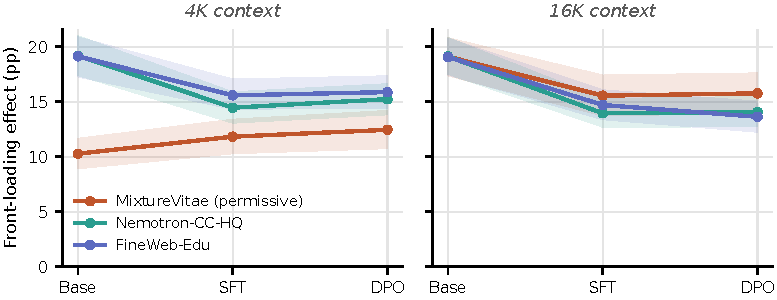
\includegraphics[width=\linewidth]{figures/frontloading_trajectory.pdf}
\caption{Front-loading effect on the reasoning suite average across post-training stages,
with 95\% paired item-level bootstrap intervals. Protocol~A.}
\label{fig:fl_trajectory}
\end{figure}

\begin{figure}[t]
\centering
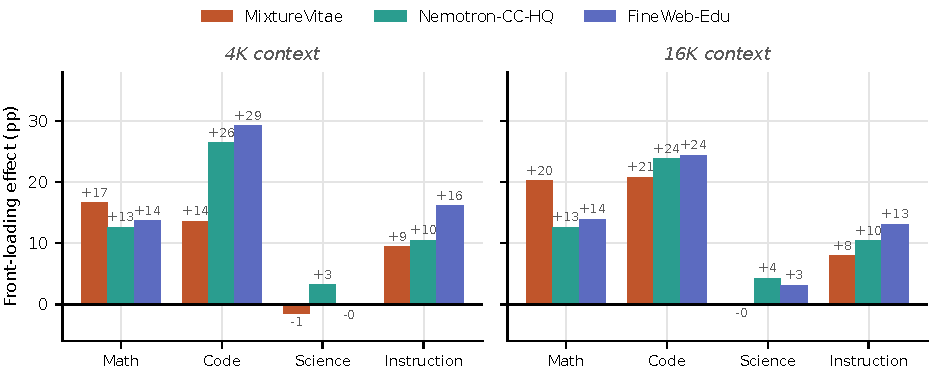
\includegraphics[width=\linewidth]{figures/frontloading_domains.pdf}
\caption{Front-loading effect by capability domain after Tulu3 SFT. The gain is broad
rather than confined to mathematics, and instruction following improves for every
substrate. Protocol~A.}
\label{fig:domains}
\end{figure}

\subsection{Reasoning post-training endpoints}
\label{app:phase2}

Table~\ref{tab:phase2_endpoints} gives the per-benchmark endpoints behind
Figure~\ref{fig:receptivity}, with each block's first row the starting checkpoint that the
OpenThoughts3-30K run was initialised from and re-evaluated under Protocol~B, so that
every comparison inside the table is paired. Table~\ref{tab:heldout_mv_grid} gives the
full held-out reasoning grid, four reasoning corpora applied from three starting
checkpoints with recipe, sample budget, and epoch count held fixed. Two observations that
the compact main-text version omits. Superior-Reasoning is a mixed control rather than a
failure, improving mathematics substantially while regressing code and instruction
following enough to lower the suite average from every starting point. And the DPO
starting point is the one that preserves instruction following through reasoning
post-training, ending at $43.0$ on IFEval against $45.0$ before the update, where the SFT
starting point falls to $25.6$.

% Generated by generate_workshop_artifacts.py. Do not edit by hand.
\begin{table}[t]
\centering
\caption{Reasoning post-training endpoints. Identical OpenThoughts3-30K post-training (30K samples, 5 epochs) is applied to every model, starting from the checkpoint named in each block's first row. Starting checkpoints are re-evaluated here, so these values are paired within the table and must not be compared against the Phase~1 tables. Protocol~B, the reasoning post-training protocol (Appendix Table~\ref{tab:eval-settings-B}). Single seed, so no error bars are available.}
\label{tab:phase2_endpoints}
\scriptsize
\setlength{\tabcolsep}{3pt}
\resizebox{\linewidth}{!}{%
\begin{tabular}{lrrrrrrrrrrrr}
\toprule
\textbf{Model} & \textbf{A24} & \textbf{A25} & \textbf{AMC} & \textbf{M500} & \textbf{GSM8K} & \textbf{HE} & \textbf{LCB} & \textbf{MBPP} & \textbf{GPQA} & \textbf{JEE} & \textbf{IFE} & \textbf{Avg} \\
\midrule
MV-16k (base) & 0.0 & 10.0 & 30.0 & 33.6 & 58.4 & 48.2 & 11.7 & 41.0 & 26.3 & 8.3 & 42.6 & 28.2 \\
\quad $\to$ SFT $\to$ OT30K & 20.0 & 16.7 & 29.8 & 72.8 & 52.5 & 58.5 & 10.0 & 29.2 & 36.4 & 4.6 & 25.6 & 32.4 \\
\quad $\to$ DPO $\to$ OT30K & 10.0 & 6.7 & 20.0 & 36.4 & 51.4 & 46.3 & 11.9 & 40.8 & 26.8 & 11.5 & 43.0 & 27.7 \\
\quad $\to$ OT30K \textbf{(no Phase 1)} & 20.0 & 16.7 & 25.0 & 71.4 & 58.9 & 57.3 & 10.0 & 31.6 & 26.3 & 6.0 & 26.6 & 31.8 \\
\midrule
FineWeb-Edu-16k $\to$ SFT & 0.0 & 0.0 & 2.5 & 1.4 & 8.5 & 2.4 & 0.3 & 2.2 & 30.3 & 3.0 & 27.6 & 7.1 \\
\quad $\to$ OT30K & 0.0 & 0.0 & 0.0 & 0.8 & 9.2 & 0.0 & 0.0 & 0.0 & 23.7 & 0.0 & 17.8 & 4.7 \\
\midrule
Nemotron-16k $\to$ SFT & 0.0 & 0.0 & 2.5 & 1.4 & 6.4 & 1.5 & 0.2 & 0.2 & 25.9 & 3.3 & 36.5 & 7.1 \\
\quad $\to$ OT30K & 0.0 & 0.0 & 0.0 & 0.4 & 5.3 & 0.0 & 0.0 & 0.2 & 21.2 & 0.2 & 20.0 & 4.3 \\
\midrule
Comma0.1-16k $\to$ SFT & 0.0 & 0.0 & 5.0 & 2.2 & 5.8 & 12.8 & 0.8 & 23.6 & 30.3 & 5.0 & 35.4 & 11.0 \\
\quad $\to$ OT30K & 0.0 & 0.0 & 0.0 & 1.6 & 14.0 & 1.8 & 0.0 & 0.0 & 28.8 & 0.0 & 20.0 & 6.0 \\
\midrule
SmolLM2-16k $\to$ SFT & 0.0 & 3.3 & 2.5 & 6.6 & 31.9 & 28.7 & 3.3 & 37.4 & 25.8 & 6.5 & 45.0 & 17.4 \\
\quad $\to$ OT30K & 0.0 & 0.0 & 0.0 & 14.0 & 26.3 & 23.2 & 0.5 & 15.8 & 27.3 & 3.3 & 34.0 & 13.1 \\
\midrule
Qwen2.5 $\to$ SFT & 0.0 & 0.0 & 7.5 & 19.6 & 39.7 & 48.2 & 3.8 & 44.6 & 22.7 & 7.5 & 44.4 & 21.6 \\
\quad $\to$ OT30K & 10.0 & 6.7 & 15.0 & 49.2 & 56.9 & 20.7 & 1.4 & 8.4 & 25.8 & 2.1 & 27.6 & 20.3 \\
\midrule
Qwen3 $\to$ SFT & 10.0 & 0.0 & 12.5 & 23.0 & 69.2 & 64.6 & 3.8 & 55.8 & 25.8 & 11.7 & 53.2 & 30.0 \\
\quad $\to$ OT30K & 0.0 & 0.0 & 0.0 & 10.6 & 29.0 & 7.3 & 1.1 & 10.6 & 28.3 & 0.5 & 30.4 & 10.7 \\
\bottomrule
\end{tabular}}
\end{table}


% Generated by generate_workshop_artifacts.py. Do not edit by hand.
\begin{table}[t]
\centering
\caption{Full held-out reasoning grid for MixtureVitae: four reasoning corpora applied from three starting checkpoints, with recipe, sample budget, and epoch count held fixed so that only the identity of the reasoning corpus changes. ``--'' marks a benchmark that was not evaluated, and that row's average is taken over the remaining ten. Protocol~B, the reasoning post-training protocol (Appendix Table~\ref{tab:eval-settings-B}). Single seed, so no error bars are available.}
\label{tab:heldout_mv_grid}
\scriptsize
\setlength{\tabcolsep}{3pt}
\resizebox{\linewidth}{!}{%
\begin{tabular}{lrrrrrrrrrrrr}
\toprule
\textbf{Reasoning corpus} & \textbf{A24} & \textbf{A25} & \textbf{AMC} & \textbf{M500} & \textbf{GSM8K} & \textbf{HE} & \textbf{LCB} & \textbf{MBPP} & \textbf{GPQA} & \textbf{JEE} & \textbf{IFE} & \textbf{Avg} \\
\midrule
\multicolumn{13}{l}{\emph{Starting from the post-YaRN base checkpoint}} \\
\quad \emph{starting checkpoint} & 0.0 & 10.0 & 30.0 & 33.6 & 58.6 & 48.2 & 11.7 & 41.0 & 26.3 & 8.3 & 42.6 & 28.2 \\
\quad OpenThoughts3 & 20.0 & 16.7 & 25.0 & 70.2 & 59.1 & 57.3 & 10.0 & 31.6 & 26.3 & 6.0 & 26.6 & 31.7~{\scriptsize($+3.5$)} \\
\quad AceReason & 3.3 & 13.3 & 30.0 & 69.2 & 61.8 & 52.4 & 9.8 & 35.6 & 26.3 & 10.4 & 24.6 & 30.6~{\scriptsize($+2.4$)} \\
\quad Nemotron-Cascade & 3.3 & 6.7 & 27.5 & 70.0 & 60.0 & 49.4 & 11.4 & 35.8 & 26.8 & 10.2 & 29.0 & 30.0~{\scriptsize($+1.8$)} \\
\quad Superior-Reasoning & 3.3 & 3.3 & 20.0 & 51.0 & 62.5 & 35.4 & 6.5 & 12.2 & 28.3 & 4.2 & 26.4 & 23.0~{\scriptsize($-5.2$)} \\
\midrule
\multicolumn{13}{l}{\emph{Starting from the Tulu3 SFT checkpoint}} \\
\quad \emph{starting checkpoint} & 0.0 & 0.0 & 5.0 & 35.2 & 51.0 & 45.1 & 8.1 & 40.2 & 28.3 & 6.5 & 41.8 & 23.8 \\
\quad OpenThoughts3 & 6.7 & 10.0 & 20.0 & 70.6 & 50.7 & 58.5 & 10.0 & 29.2 & 36.4 & 4.6 & 25.6 & 29.3~{\scriptsize($+5.5$)} \\
\quad AceReason & 3.3 & 20.0 & 25.0 & 69.4 & 54.4 & 48.2 & 10.8 & 33.6 & 27.3 & 9.9 & 25.6 & 29.8~{\scriptsize($+6.0$)} \\
\quad Nemotron-Cascade & 3.3 & 13.3 & 27.5 & 66.8 & 52.6 & 50.6 & -- & 32.8 & 34.8 & 7.3 & 30.6 & 32.0~{\scriptsize($+8.2$)} \\
\quad Superior-Reasoning & 6.7 & 3.3 & 20.0 & 51.6 & 55.6 & 22.0 & 6.2 & 15.6 & 25.8 & 4.9 & 27.0 & 21.7~{\scriptsize($-2.1$)} \\
\midrule
\multicolumn{13}{l}{\emph{Starting from the Tulu3 SFT + DPO checkpoint}} \\
\quad \emph{starting checkpoint} & 0.0 & 0.0 & 2.5 & 33.2 & 51.9 & 47.6 & 8.7 & 40.4 & 27.8 & 8.9 & 45.0 & 24.2 \\
\quad OpenThoughts3 & 10.0 & 6.7 & 20.0 & 36.4 & 50.7 & 44.5 & 11.9 & 40.8 & 26.8 & 11.5 & 43.0 & 27.5~{\scriptsize($+3.3$)} \\
\quad AceReason & 6.7 & 16.7 & 27.5 & 70.8 & 55.4 & 48.2 & 11.4 & 32.6 & 23.7 & 9.8 & 25.0 & 29.8~{\scriptsize($+5.6$)} \\
\quad Nemotron-Cascade & 6.7 & 10.0 & 25.0 & 68.2 & 53.5 & 50.0 & 13.3 & 34.8 & 28.8 & 9.7 & 30.4 & 30.0~{\scriptsize($+5.8$)} \\
\quad Superior-Reasoning & 3.3 & 6.7 & 20.0 & 54.2 & 55.1 & 28.7 & 5.7 & 13.2 & 24.7 & 5.3 & 28.0 & 22.3~{\scriptsize($-1.9$)} \\
\bottomrule
\end{tabular}}
\end{table}


\subsection{Mixture composition at a 100B budget}
\label{app:mixture100b}

Tables~\ref{tab:evalchemy_table1} and~\ref{tab:lang_eval_table1} give the per-benchmark
values behind the mixture-composition ablation of Section~\ref{sec:zoo}, in which two
ablated variants of the permissive mixture are pre-trained at 100B tokens and passed
through the same Phase 1 pipeline. Removing the instruction-and-reasoning subset collapses
performance across mathematics, code, and reasoning at both context lengths, with AIME24
and AIME25 at zero, MATH500 below three, and suite averages of $6.1$ to $8.5$ at 4K and
$6.7$ to $7.5$ at 16K, and Tulu3 SFT does not repair it. Removing the curated web subset
behaves very differently, reaching $18.6$ at the 4K base and $16.1$ to $17.5$ after Phase
1, never below the full mixture and above it on MATH500, AMC23, HumanEval, and MBPP. On
language understanding the web ablation costs about a point, $49.0$ to $50.0$ mean
accuracy against $50.0$ to $51.0$ for the full mixture, while the instruction ablation
costs 4 to 5 points that Phase 1 does not close. We state this for the scale and budget
tested and do not generalise it.

\subsection{Smaller scale check at 0.4B}
\label{app:smallscale}

Tables~\ref{tab:evalchemy_table4} and~\ref{tab:lang_eval_table4} compare a 0.4B permissive
model against Baguettotron, a 0.32B model trained on the PleIAs SYNTH
mix~\citep{synthpleias2025}, under the same Phase 1 pipeline. The permissive model reaches $12.1$ reasoning suite average after DPO against $6.2$ for Baguettotron, with HumanEval and
MBPP pass@1 of $15.3$ and $22.6$ against near zero, and $45.0$ against $42.0$ to $43.0$
mean accuracy on the language suite. The decontamination status of the SYNTH mix is
undocumented while our model is decontaminated against every benchmark reported here, so
some part of Baguettotron's score may reflect train and test overlap that we cannot rule
out from outside the release. This comparison is a sanity check on the direction of the
effect at a second scale and not a scaling result.


\begin{table}[ht]
\centering
\caption{Per-benchmark results for the 100B-token MixtureVitae mixture-composition ablation on the primary reasoning suite. Removing the instruction-and-reasoning subset causes a broad collapse in math, code, and reasoning that Phase 1 Tulu3 SFT/DPO does not recover, whereas removing the curated web subset leaves performance comparable to, and on several benchmarks stronger than, the full mixture at both 4K and 16K context. Bold marks the column maximum.}
\label{tab:evalchemy_table1}
\scriptsize
\resizebox{\columnwidth}{!}{%
\begin{tabular}{lrrrrrrrrrrrr}
\toprule
\textbf{Model} & \textbf{A24} & \textbf{A25} & \textbf{AMC} & \textbf{M500} & \textbf{GSM8K} & \textbf{HE} & \textbf{LCB} & \textbf{MBPP} & \textbf{GPQA} & \textbf{JEE} & \textbf{IFE} & \textbf{Avg} \\
\midrule
MV-noinstruct & 0.0 & 0.0 & 0.0 & 0.4 & 2.6 & 0.6 & 0.0 & 14.2 & 23.9 & 0.0 & 24.8 & 6.1 \\
\quad $\to$ SFT & 0.0 & 0.0 & 2.5 & 1.8 & 4.2 & 7.3 & 1.0 & 15.8 & 20.7 & 3.4 & 29.9 & 7.9 \\
\quad $\to$ SFT $\to$ DPO & 0.0 & 0.0 & 2.5 & 2.0 & 3.8 & 7.0 & 1.4 & 15.2 & 25.1 & 4.0 & 32.0 & 8.5 \\
\midrule
\addlinespace[0.3em]
MV-noinstruct-16k & 0.0 & 0.0 & 2.5 & 1.6 & 4.2 & 1.5 & 0.0 & 2.0 & 24.6 & 4.7 & 32.9 & 6.7 \\
\quad $\to$ SFT & 0.0 & 0.0 & 0.0 & 2.2 & 4.8 & 3.4 & 0.4 & 3.4 & \textbf{25.6} & 2.1 & 35.2 & 7.0 \\
\quad $\to$ SFT $\to$ DPO & 0.0 & 0.0 & 2.5 & 2.6 & 5.2 & 4.9 & 0.6 & 4.8 & 23.7 & 2.2 & 36.0 & 7.5 \\
\midrule
\addlinespace[0.3em]
MV-noweb & 0.0 & 0.0 & 17.5 & 26.4 & 42.4 & 23.5 & \textbf{7.4} & 34.6 & 23.7 & 2.6 & 26.5 & \textbf{18.6} \\
\quad $\to$ SFT & 0.0 & 0.0 & 7.5 & 10.0 & 36.0 & 23.6 & 2.4 & 36.8 & 22.4 & 3.7 & 35.0 & 16.1 \\
\quad $\to$ SFT $\to$ DPO & 0.0 & \textbf{3.3} & 10.0 & 12.2 & 36.5 & \textbf{25.1} & 1.8 & \textbf{38.0} & 25.2 & 4.3 & 36.2 & 17.5 \\
\midrule
\addlinespace[0.3em]
MV-noweb-16k & 0.0 & 0.0 & 10.0 & 35.0 & \textbf{44.7} & 10.7 & 3.5 & 9.0 & 23.9 & 4.4 & 37.4 & 16.2 \\
\quad $\to$ SFT & 0.0 & 0.0 & 7.5 & 18.2 & 33.6 & 9.5 & 3.5 & 7.2 & 22.1 & 4.3 & 38.2 & 13.1 \\
\quad $\to$ SFT $\to$ DPO & \textbf{3.3} & \textbf{3.3} & \textbf{20.0} & 21.2 & 35.0 & 11.0 & 3.3 & 7.8 & 21.0 & 2.9 & 38.3 & 15.2 \\
\midrule
\addlinespace[0.3em]
MV & \textbf{3.3} & 0.0 & 0.0 & 12.2 & 42.1 & 0.6 & 0.0 & 0.2 & 24.4 & 3.2 & 21.2 & 9.8 \\
\quad $\to$ SFT & 0.0 & 0.0 & 5.0 & 6.6 & 38.4 & 22.3 & 3.3 & 36.8 & 20.7 & 2.5 & 34.9 & 15.5 \\
\quad $\to$ SFT $\to$ DPO & 0.0 & 0.0 & 5.0 & 8.0 & 39.2 & 22.6 & 4.3 & 36.4 & 24.4 & 2.9 & 35.1 & 16.2 \\
\midrule
\addlinespace[0.3em]
MV-16k & 0.0 & 0.0 & 17.5 & \textbf{35.2} & 40.6 & 2.5 & 3.7 & 7.2 & 22.4 & \textbf{7.2} & 40.4 & 16.1 \\
\quad $\to$ SFT & 0.0 & 0.0 & 0.0 & 3.2 & 36.5 & 11.6 & 0.6 & 6.4 & 23.9 & 4.4 & 39.5 & 11.5 \\
\quad $\to$ SFT $\to$ DPO & 0.0 & 0.0 & 0.0 & 3.4 & 36.4 & 0.9 & 0.8 & 8.2 & 24.6 & 4.0 & \textbf{41.6} & 10.9 \\
\bottomrule
\end{tabular}
}
\end{table}


\begin{table}[ht]
\centering
\caption{Reasoning-suite comparison between decontaminated and non-decontaminated 300B MixtureVitae checkpoints at 4K and 16K context, before and after Phase 1 Tulu3 SFT/DPO. Decontamination changes some base scores, but the post-training picture remains the same: the gains reported in the main paper persist after decontamination. Bold marks the column maximum.}
\label{tab:evalchemy_table3}
\resizebox{\textwidth}{!}{%
\scriptsize
\begin{tabular}{llrrrrrrrrrrrr}
\toprule
\textbf{Base} & \textbf{Model} & \textbf{A24} & \textbf{A25} & \textbf{AMC} & \textbf{M500} & \textbf{GSM8K} & \textbf{HE} & \textbf{LCB} & \textbf{MBPP} & \textbf{GPQA} & \textbf{JEE} & \textbf{IFE} & \textbf{Avg}  \\
\midrule
\multirow{6}{*}{Not Decontaminated} & MV & 0.0 & 0.0 & 15.0 & 14.6 & 53.1 & 26.6 & 11.2 & 43.0 & 22.2 & 5.0 & 27.8 & 19.9 \\
 & \quad $\to$ SFT & \textbf{6.7} & 0.0 & 2.5 & 16.4 & 50.6 & 32.5 & 11.2 & 42.6 & 25.6 & 3.5 & 45.0 & 21.5 \\
 & \quad $\to$ SFT $\to$ DPO & 0.0 & 0.0 & 7.5 & 17.6 & 50.9 & 32.8 & 12.5 & 43.0 & \textbf{27.8} & 3.5 & 46.7 & 22.0 \\
\cmidrule{2-14}
 & MV-16k & 3.3 & 6.7 & 20.0 & 36.6 & \textbf{61.8} & 30.0 & 16.8 & 41.8 & 22.6 & \textbf{11.0} & 47.9 & 27.1 \\
 & \quad $\to$ SFT & 0.0 & 0.0 & 5.0 & 18.0 & 51.3 & 29.7 & 10.6 & \textbf{43.2} & 27.3 & 2.7 & 49.5 & 21.6 \\
 & \quad $\to$ SFT $\to$ DPO & 0.0 & 0.0 & 0.0 & 18.0 & 51.5 & 30.0 & 11.0 & 41.8 & 25.2 & 3.8 & \textbf{50.7} & 21.1 \\
\midrule
\addlinespace[0.3em]
\multirow{6}{*}{Decontaminated} & MV & 0.0 & \textbf{10.0} & 7.5 & 17.4 & 53.5 & 11.7 & 12.7 & 18.6 & 23.9 & 4.1 & 25.6 & 16.8 \\
 & \quad $\to$ SFT & 0.0 & 0.0 & 7.5 & 28.6 & 49.3 & 27.9 & 2.1 & 41.2 & 26.1 & 4.2 & 42.4 & 20.8 \\
 & \quad $\to$ SFT $\to$ DPO & 0.0 & 0.0 & 15.0 & 27.4 & 50.5 & 27.9 & 1.8 & 40.8 & 24.6 & 3.1 & 42.9 & 21.3 \\
\cmidrule{2-14}
 & MV-16k & 0.0 & 0.0 & \textbf{27.5} & \textbf{46.0} & 58.6 & 31.9 & \textbf{22.7} & 39.8 & 25.2 & 8.2 & 46.9 & \textbf{27.9} \\
 & \quad $\to$ SFT & 3.3 & 0.0 & 12.5 & 31.0 & 51.9 & \textbf{33.2} & 15.5 & 40.6 & 23.4 & 5.2 & 47.1 & 24.0 \\
 & \quad $\to$ SFT $\to$ DPO & \textbf{6.7} & 0.0 & 15.0 & 33.6 & 52.1 & \textbf{33.2} & 14.9 & 40.0 & 25.2 & 5.4 & 49.5 & 25.0 \\
\bottomrule
\end{tabular}
}
\end{table}


\begin{table}[ht]
\centering
\caption{Reasoning-suite results for the smaller-scale comparison between MV (0.4B) and Baguettotron. Across 4K and 16K context, MV is substantially more receptive to Phase 1 post-training, especially on code and broader reasoning, while Baguettotron remains weak throughout. Bold marks the column maximum.}
\label{tab:evalchemy_table4}
\scriptsize
\resizebox{\columnwidth}{!}{%
\begin{tabular}{lrrrrrrrrrrrr}
\toprule
\textbf{Model} & \textbf{A24} & \textbf{A25} & \textbf{AMC} & \textbf{M500} & \textbf{GSM8K} & \textbf{HE} & \textbf{LCB} & \textbf{MBPP} & \textbf{GPQA} & \textbf{JEE} & \textbf{IFE} & \textbf{Avg} \\
\midrule
Baguettotron & 0.0 & \textbf{0.0} & 0.0 & 0.2 & 2.3 & 0.0 & 0.0 & 0.0 & 23.1 & 0.2 & 24.3 & 4.5 \\
\quad $\to$ SFT & 0.0 & \textbf{0.0} & 2.5 & 2.0 & 7.7 & 0.0 & 0.0 & 0.0 & 24.4 & 1.3 & 26.9 & 5.9 \\
\quad $\to$ SFT $\to$ DPO & 0.0 & \textbf{0.0} & 0.0 & 2.8 & 8.3 & 0.0 & 0.0 & 0.0 & \textbf{26.3} & 1.1 & 30.2 & 6.2 \\
\midrule
\addlinespace[0.3em]
Baguettotron 16k & 0.0 & \textbf{0.0} & 0.0 & 2.0 & 5.2 & 0.6 & 0.0 & 0.0 & 21.6 & 1.8 & \textbf{34.2} & 5.9 \\
\quad $\to$ SFT & 0.0 & \textbf{0.0} & 2.5 & 2.4 & 8.1 & 0.0 & 0.0 & 0.0 & 24.4 & 1.1 & 30.0 & 6.2 \\
\quad $\to$ SFT $\to$ DPO & 0.0 & \textbf{0.0} & 2.5 & 3.2 & 8.7 & 0.0 & 0.0 & 0.0 & 24.9 & 1.5 & 31.8 & 6.6 \\
\midrule
\addlinespace[0.3em]
MV (0.4B) & \textbf{3.3} & \textbf{0.0} & 2.5 & 0.6 & 28.7 & 1.2 & 1.0 & 5.2 & 22.4 & 1.1 & 19.6 & 7.8 \\
\quad $\to$ SFT & 0.0 & \textbf{0.0} & 2.5 & 6.2 & 23.1 & 0.6 & 7.0 & 12.2 & 25.6 & 1.7 & 27.1 & 9.6 \\
\quad $\to$ SFT $\to$ DPO & 0.0 & \textbf{0.0} & 2.5 & 7.4 & 23.1 & \textbf{15.3} & \textbf{8.2} & \textbf{22.6} & 24.1 & 2.3 & 28.1 & 12.1 \\
\midrule
\addlinespace[0.3em]
MV-16k (0.4B) & 0.0 & \textbf{0.0} & \textbf{7.5} & \textbf{19.8} & \textbf{29.5} & 6.4 & 0.8 & 13.8 & 22.2 & \textbf{4.3} & 32.6 & \textbf{12.4} \\
\quad $\to$ SFT & 0.0 & \textbf{0.0} & 2.5 & 6.2 & 24.5 & 8.9 & 1.4 & 13.6 & 22.9 & 2.3 & 29.9 & 10.2 \\
\quad $\to$ SFT $\to$ DPO & 0.0 & \textbf{0.0} & 2.5 & 6.8 & 24.9 & 7.7 & 1.6 & 11.2 & 23.1 & 2.6 & 31.4 & 10.1 \\
\bottomrule
\end{tabular}}

\end{table}


\begin{table}[htbp]
\centering
\caption{Per-benchmark results for the 100B token MixtureVitae mixture composition ablation on the standard language understanding suite. Removing the instruction and reasoning subset creates a persistent language gap that Phase 1 does not close, whereas removing the curated web subset leaves language performance close to the full mixture across stages and both context lengths. Bold marks the column maximum.}
\label{tab:lang_eval_table1}
\scriptsize
\resizebox{\columnwidth}{!}{%
\begin{tabular}{lrrrrrrrrrrrr}
\toprule
\textbf{Model} & \textbf{ARC-C} & \textbf{ARC-E} & \textbf{BoolQ} & \textbf{CSQA} & \textbf{COPA} & \textbf{HellaS} & \textbf{LAMBADA} & \textbf{MMLU} & \textbf{OBQA} & \textbf{PIQA} & \textbf{WinoG} & \textbf{Avg} \\
\midrule
MV-noinstruct & 32.0 & 61.0 & 58.0 & 18.0 & 66.0 & 46.0 & 46.0 & 25.0 & 33.0 & 68.0 & 55.0 & 46.0 \\
\quad $\to$SFT & 32.0 & 61.0 & 57.0 & 19.0 & 66.0 & 46.0 & \textbf{47.0} & 25.0 & 33.0 & 68.0 & 55.0 & 46.0 \\
\quad $\to$SFT $\to$DPO & 32.0 & 61.0 & 57.0 & 19.0 & 66.0 & 47.0 & \textbf{47.0} & 25.0 & 33.0 & 68.0 & 55.0 & 46.0 \\
\midrule
\addlinespace[0.3em]
MV-noinstruct-16k & 33.0 & 60.0 & 63.0 & 19.0 & 69.0 & 46.0 & \textbf{47.0} & 25.0 & 33.0 & 67.0 & 55.0 & 47.0 \\
\quad $\to$SFT & 31.0 & 60.0 & 61.0 & 18.0 & 67.0 & 46.0 & \textbf{47.0} & 25.0 & 33.0 & 67.0 & 56.0 & 46.0 \\
\quad $\to$SFT $\to$DPO & 31.0 & 60.0 & 61.0 & 18.0 & 67.0 & 47.0 & \textbf{47.0} & 25.0 & 32.0 & 67.0 & 56.0 & 46.0 \\
\midrule
\addlinespace[0.3em]
MV-noweb & 34.0 & \textbf{65.0} & 67.0 & 35.0 & 67.0 & 46.0 & 39.0 & 31.0 & 33.0 & 68.0 & 56.0 & 49.0 \\
\quad $\to$SFT & 33.0 & 63.0 & 65.0 & 35.0 & 69.0 & 47.0 & 41.0 & \textbf{33.0} & 32.0 & 67.0 & 55.0 & 49.0 \\
\quad $\to$SFT $\to$DPO & 33.0 & 63.0 & 65.0 & 35.0 & 69.0 & 47.0 & 41.0 & \textbf{33.0} & 32.0 & 67.0 & 55.0 & 49.0 \\
\midrule
\addlinespace[0.3em]
MV-noweb-16k & \textbf{36.0} & \textbf{65.0} & 70.0 & \textbf{37.0} & \textbf{70.0} & 45.0 & 40.0 & 32.0 & 32.0 & 67.0 & 56.0 & 50.0 \\
\quad $\to$SFT & 33.0 & 63.0 & 66.0 & 34.0 & 69.0 & 46.0 & 41.0 & \textbf{33.0} & 33.0 & 67.0 & 56.0 & 49.0 \\
\quad $\to$SFT $\to$DPO & 33.0 & 63.0 & 67.0 & 34.0 & 69.0 & 47.0 & 41.0 & \textbf{33.0} & 33.0 & 67.0 & 56.0 & 49.0 \\
\midrule
\addlinespace[0.3em]
MV & 34.0 & \textbf{65.0} & \textbf{71.0} & 31.0 & 67.0 & 48.0 & 44.0 & 32.0 & \textbf{34.0} & 68.0 & 58.0 & 50.0 \\
\quad $\to$SFT & 34.0 & 64.0 & \textbf{71.0} & 32.0 & 69.0 & \textbf{49.0} & 45.0 & \textbf{33.0} & \textbf{34.0} & \textbf{69.0} & 58.0 & \textbf{51.0} \\
\quad $\to$SFT $\to$DPO & 34.0 & 64.0 & \textbf{71.0} & 32.0 & \textbf{70.0} & \textbf{49.0} & 45.0 & \textbf{33.0} & 33.0 & \textbf{69.0} & 58.0 & \textbf{51.0} \\
\midrule
\addlinespace[0.3em]
MV-16k & 35.0 & \textbf{65.0} & 68.0 & 30.0 & 67.0 & 47.0 & 45.0 & \textbf{33.0} & 33.0 & 68.0 & 57.0 & 50.0 \\
\quad $\to$SFT & 33.0 & 64.0 & 69.0 & 29.0 & 68.0 & \textbf{49.0} & 45.0 & 32.0 & 33.0 & 68.0 & \textbf{59.0} & 50.0 \\
\quad $\to$SFT $\to$DPO & 33.0 & 64.0 & 69.0 & 30.0 & 68.0 & \textbf{49.0} & 45.0 & 32.0 & 33.0 & 68.0 & \textbf{59.0} & 50.0 \\
\bottomrule
\end{tabular}
}
\end{table}


\begin{table}[htbp]
\centering
\caption{Full language suite results for the main 1.7B comparison. Phase 1 Tulu3 SFT/DPO leaves language scores largely unchanged, with MixtureVitae matching FineWeb-Edu, trailing Nemotron, and remaining below the more heavily pretrained external baselines. Bold marks the column maximum.}
\label{tab:lang_eval_table2}
\resizebox{\textwidth}{!}{%
\scriptsize
\begin{tabular}{lrrrrrrrrrrrr}
\toprule
Model & ARC-C & ARC-E & BoolQ & CSQA & COPA & HellaS & LAMBADA & MMLU & OBQA & PIQA & WinoG & Avg  \\
\midrule
Comma0.1-300BT       & 36.0 & 63.0 & 62.0 & 21.0 & 71.0 & 53.0 & 54.0 & 27.0 & 33.0 & 71.0 & 60.0 & 50.0 \\
\quad $\to$SFT & 37.0 & 65.0 & 64.0 & 20.0 & 74.0 & 54.0 & 57.0 & 27.0 & 33.0 & 72.0 & 61.0 & 51.0 \\
\quad $\to$SFT $\to$DPO & 37.0 & 65.0 & 65.0 & 20.0 & 74.0 & 54.0 & 57.0 & 27.0 & 33.0 & 72.0 & 61.0 & 51.0 \\
\midrule
\addlinespace[0.3em]
MV          & 40.0 & 71.0 & 74.0 & 51.0 & 71.0 & 54.0 & 48.0 & 42.0 & 34.0 & 70.0 & 58.0 & 56.0 \\
\quad $\to$SFT & 39.0 & 70.0 & 73.0 & 50.0 & 70.0 & 56.0 & 50.0 & 43.0 & 34.0 & 70.0 & 58.0 & 56.0 \\
\quad $\to$SFT $\to$DPO & 39.0 & 70.0 & 73.0 & 50.0 & 71.0 & 56.0 & 50.0 & 43.0 & 34.0 & 70.0 & 58.0 & 56.0 \\
\midrule
\addlinespace[0.3em]
MV-16k          & 42.0 & 71.0 & 73.0 & 49.0 & 67.0 & 53.0 & 49.0 & 41.0 & 32.0 & 70.0 & 58.0 & 55.0 \\
\quad $\to$SFT & 39.0 & 70.0 & 73.0 & 50.0 & 69.0 & 55.0 & 50.0 & 42.0 & 34.0 & 70.0 & 57.0 & 55.0 \\
\quad $\to$SFT $\to$DPO & 39.0 & 71.0 & 73.0 & 50.0 & 69.0 & 55.0 & 50.0 & 42.0 & 34.0 & 70.0 & 57.0 & 55.0 \\
\midrule
\addlinespace[0.3em]
Qwen2.5-1.5B       & \textbf{54.0} & 81.0 & 78.0 & 76.0 & 83.0 & 68.0 & 62.0 & 61.0 & 40.0 & 77.0 & 63.0 & \textbf{68.0} \\
\quad $\to$SFT & 51.0 & 79.0 & 70.0 & \textbf{77.0} & 82.0 & 68.0 & 60.0 & 60.0 & 40.0 & 77.0 & 63.0 & 66.0 \\
\quad $\to$SFT $\to$DPO & 52.0 & 79.0 & 70.0 & 76.0 & 82.0 & 68.0 & 60.0 & 60.0 & 39.0 & 77.0 & 63.0 & 66.0 \\
\midrule
\addlinespace[0.3em]
Qwen3-1.7B       & \textbf{54.0} & \textbf{82.0} & \textbf{83.0} & 76.0 & 82.0 & 67.0 & 63.0 & \textbf{63.0} & 38.0 & 76.0 & 64.0 & \textbf{68.0} \\
\quad $\to$SFT & 53.0 & 81.0 & 82.0 & \textbf{77.0} & 80.0 & 68.0 & 61.0 & \textbf{63.0} & 39.0 & 76.0 & 64.0 & \textbf{68.0} \\
\quad $\to$SFT $\to$DPO & 53.0 & 81.0 & \textbf{83.0} & \textbf{77.0} & 80.0 & 68.0 & 61.0 & \textbf{63.0} & 39.0 & 76.0 & 64.0 & \textbf{68.0} \\
\midrule
\addlinespace[0.3em]
SmolLM2-1.7B       & \textbf{54.0} & 80.0 & 75.0 & 60.0 & 82.0 & 73.0 & 67.0 & 50.0 & \textbf{44.0} & \textbf{79.0} & \textbf{67.0} & 66.0 \\
\quad $\to$SFT & 53.0 & 80.0 & 75.0 & 61.0 & \textbf{85.0} & \textbf{74.0} & \textbf{69.0} & 49.0 & 43.0 & \textbf{79.0} & \textbf{67.0} & 67.0 \\
\quad $\to$SFT $\to$DPO & \textbf{54.0} & 80.0 & 75.0 & 61.0 & \textbf{85.0} & \textbf{74.0} & \textbf{69.0} & 49.0 & 43.0 & \textbf{79.0} & \textbf{67.0} & 67.0 \\
\midrule
\addlinespace[0.3em]
FineWeb-Edu-300BT & 48.0 & 77.0 & 65.0 & 21.0 & 82.0 & 67.0 & 56.0 & 26.0 & 42.0 & 77.0 & 62.0 & 57.0 \\
\quad $\to$SFT & 48.0 & 79.0 & 66.0 & 20.0 & 83.0 & 68.0 & 59.0 & 27.0 & 42.0 & 77.0 & 63.0 & 57.0 \\
\quad $\to$SFT $\to$DPO & 48.0 & 78.0 & 66.0 & 20.0 & 83.0 & 68.0 & 59.0 & 27.0 & 42.0 & 77.0 & 63.0 & 57.0 \\
\midrule
\addlinespace[0.3em]
Nemotron       & 52.0 & 81.0 & 77.0 & 49.0 & \textbf{85.0} & 71.0 & 58.0 & 46.0 & 42.0 & \textbf{79.0} & 65.0 & 64.0 \\
\quad $\to$SFT & 48.0 & 79.0 & 74.0 & 46.0 & 82.0 & 70.0 & 58.0 & 43.0 & 43.0 & 78.0 & 65.0 & 62.0 \\
\quad $\to$SFT $\to$DPO & 48.0 & 79.0 & 74.0 & 46.0 & 82.0 & 71.0 & 59.0 & 43.0 & 43.0 & 78.0 & 65.0 & 63.0 \\
\midrule
\bottomrule
\end{tabular}%
}
\end{table}


\begin{table}[htbp]
\centering
\caption{Language suite comparison between decontaminated and non-decontaminated 300B MixtureVitae checkpoints at 4K and 16K context, before and after Phase 1 Tulu3 SFT/DPO. In contrast to the reasoning suite, the language results are essentially unchanged by decontamination. Bold marks the column maximum.}
\label{tab:lang_eval_table3}
\scriptsize
\resizebox{\textwidth}{!}{%
\begin{tabular}{llrrrrrrrrrrrr}
\toprule
\textbf{Base} & \textbf{Model} & \textbf{ARC-C} & \textbf{ARC-E} & \textbf{BoolQ} & \textbf{CSQA} & \textbf{COPA} & \textbf{HellaS} & \textbf{LAMBADA} & \textbf{MMLU} & \textbf{OBQA} & \textbf{PIQA} & \textbf{WinoG} & \textbf{Avg} \\
\midrule
\multirow{6}{*}{Not Decontaminated} & MV & 40.0 & \textbf{71.0} & \textbf{75.0} & 49.0 & \textbf{73.0} & 54.0 & 48.0 & 38.0 & 35.0 & 70.0 & 58.0 & \textbf{56.0} \\
 & \quad $\to$SFT & 39.0 & 70.0 & \textbf{75.0} & 47.0 & 71.0 & 55.0 & \textbf{50.0} & 40.0 & 35.0 & 70.0 & 58.0 & 55.0 \\
 & \quad $\to$SFT $\to$DPO & 39.0 & 70.0 & \textbf{75.0} & 47.0 & 71.0 & 55.0 & \textbf{50.0} & 40.0 & 35.0 & 70.0 & 58.0 & \textbf{56.0} \\
\cmidrule{2-14}
 & MV-16k & 39.0 & \textbf{71.0} & \textbf{75.0} & 50.0 & 72.0 & 54.0 & 49.0 & 38.0 & \textbf{36.0} & \textbf{71.0} & 58.0 & \textbf{56.0} \\
 & \quad $\to$SFT & 39.0 & \textbf{71.0} & 74.0 & 48.0 & 72.0 & 55.0 & \textbf{50.0} & 38.0 & 35.0 & 70.0 & \textbf{59.0} & 55.0 \\
 & \quad $\to$SFT $\to$DPO & 39.0 & \textbf{71.0} & 74.0 & 48.0 & 72.0 & 55.0 & \textbf{50.0} & 38.0 & 35.0 & \textbf{71.0} & \textbf{59.0} & \textbf{56.0} \\
\midrule
\addlinespace[0.3em]
\multirow{6}{*}{Decontaminated} & MV & 40.0 & \textbf{71.0} & 74.0 & \textbf{51.0} & 71.0 & 54.0 & 48.0 & 42.0 & 34.0 & 70.0 & 58.0 & \textbf{56.0} \\
 & \quad $\to$SFT & 39.0 & 70.0 & 73.0 & 50.0 & 70.0 & \textbf{56.0} & \textbf{50.0} & \textbf{43.0} & 34.0 & 70.0 & 58.0 & \textbf{56.0} \\
 & \quad $\to$SFT $\to$DPO & 39.0 & 70.0 & 73.0 & 50.0 & 71.0 & \textbf{56.0} & \textbf{50.0} & \textbf{43.0} & 34.0 & 70.0 & 58.0 & \textbf{56.0} \\
\cmidrule{2-14}
 & MV-16k & \textbf{42.0} & \textbf{71.0} & 73.0 & 49.0 & 67.0 & 53.0 & 49.0 & 41.0 & 32.0 & 70.0 & 58.0 & 55.0 \\
 & \quad $\to$SFT & 39.0 & 70.0 & 73.0 & 50.0 & 69.0 & 55.0 & \textbf{50.0} & 42.0 & 34.0 & 70.0 & 57.0 & 55.0 \\
 & \quad $\to$SFT $\to$DPO & 39.0 & \textbf{71.0} & 73.0 & 50.0 & 69.0 & 55.0 & \textbf{50.0} & 42.0 & 34.0 & 70.0 & 57.0 & 55.0 \\
\bottomrule
\end{tabular}%
}
\end{table}


\begin{table}[htbp]
\centering
\caption{Language suite results for the smaller scale comparison between MV (0.4B) and Baguettotron. MV retains a small but consistent advantage across both context lengths and post-training stages, showing that its broader general-purpose edge at small scale is not limited to reasoning tasks. Bold marks the column maximum.}
\label{tab:lang_eval_table4}
\scriptsize
\resizebox{\columnwidth}{!}{%
\begin{tabular}{lrrrrrrrrrrrr}
\toprule
\textbf{Model} & \textbf{ARC-C} & \textbf{ARC-E} & \textbf{BoolQ} & \textbf{CSQA} & \textbf{COPA} & \textbf{HellaS} & \textbf{LAMBADA} & \textbf{MMLU} & \textbf{OBQA} & \textbf{PIQA} & \textbf{WinoG} & \textbf{Avg} \\
\midrule
Baguettotron & \textbf{33.0} & 58.0 & 61.0 & 19.0 & 56.0 & 36.0 & 30.0 & 27.0 & 31.0 & 61.0 & 53.0 & 42.0 \\
\quad $\to$SFT & 30.0 & 57.0 & 61.0 & 21.0 & 61.0 & 36.0 & 33.0 & 26.0 & \textbf{32.0} & 61.0 & \textbf{55.0} & 43.0 \\
\quad $\to$SFT $\to$DPO & 31.0 & 57.0 & 62.0 & 21.0 & 61.0 & 36.0 & 33.0 & 26.0 & \textbf{32.0} & 61.0 & 54.0 & 43.0 \\
\midrule
\addlinespace[0.3em]
Baguettotron 16k & 32.0 & 58.0 & 57.0 & 21.0 & 60.0 & 36.0 & 34.0 & 26.0 & 31.0 & 61.0 & \textbf{55.0} & 43.0 \\
\quad $\to$SFT & 31.0 & 57.0 & \textbf{64.0} & 20.0 & 61.0 & 36.0 & 33.0 & 26.0 & 31.0 & 61.0 & 54.0 & 43.0 \\
\quad $\to$SFT $\to$DPO & 31.0 & 57.0 & \textbf{64.0} & 19.0 & 61.0 & 36.0 & 33.0 & 26.0 & \textbf{32.0} & 61.0 & 54.0 & 43.0 \\
\midrule
\addlinespace[0.3em]
MV (0.4B) & 32.0 & \textbf{61.0} & 60.0 & \textbf{26.0} & 63.0 & \textbf{42.0} & 38.0 & 28.0 & 31.0 & \textbf{66.0} & 53.0 & \textbf{45.0} \\
\quad $\to$SFT & 29.0 & 59.0 & 50.0 & 25.0 & 63.0 & \textbf{42.0} & 40.0 & \textbf{29.0} & 30.0 & 65.0 & 53.0 & 44.0 \\
\quad $\to$SFT $\to$DPO & 29.0 & 59.0 & 50.0 & \textbf{26.0} & 63.0 & \textbf{42.0} & 40.0 & \textbf{29.0} & 30.0 & 65.0 & 54.0 & 44.0 \\
\midrule
\addlinespace[0.3em]
MV-16k (0.4B) & 32.0 & \textbf{61.0} & 58.0 & \textbf{26.0} & 63.0 & 41.0 & \textbf{41.0} & 28.0 & \textbf{32.0} & 65.0 & 54.0 & \textbf{45.0} \\
\quad $\to$SFT & 28.0 & 59.0 & 53.0 & 25.0 & \textbf{64.0} & \textbf{42.0} & 40.0 & \textbf{29.0} & 31.0 & 65.0 & \textbf{55.0} & \textbf{45.0} \\
\quad $\to$SFT $\to$DPO & 28.0 & 59.0 & 54.0 & 25.0 & 63.0 & \textbf{42.0} & \textbf{41.0} & \textbf{29.0} & 31.0 & 65.0 & \textbf{55.0} & \textbf{45.0} \\
\bottomrule
\end{tabular}
}
\end{table}

\begin{table}[htbp]
\centering
\caption{Language suite results after Phase 2 OpenThoughts3 30K post-training for the models evaluated in the OT3 experiments. Reasoning post-training preserves general language understanding, and MV-16K performs equally well with the full pipeline or with direct OT3 post-training from the post-YaRN base. Bold marks the column maximum.}
\label{tab:lang_eval_ot3_phase2}
\resizebox{\textwidth}{!}{%
\scriptsize
\begin{tabular}{lrrrrrrrrrrrr}
\toprule
\textbf{Model} & ARC-C & ARC-E & BoolQ & CSQA & COPA & HellaS & LAMBADA & MMLU & OBQA & PIQA & WinoG & Avg  \\
\midrule
MV-16k & & & & & & & & & & & &  \\
\quad $\to$SFT $\to$DPO $\to$OT30K                  & 40.0 & 70.0 & 73.0 & 50.0 & 71.0 & 55.0 & 49.0 & 41.0 & 34.0 & 70.0 & 59.0 & 56.0 \\
\quad $\to$OT30K (\textbf{no Phase 1})        & 43.0 & 71.0 & 74.0 & 49.0 & 69.0 & 54.0 & 49.0 & 42.0 & 33.0 & 70.0 & 59.0 & 56.0 \\
\midrule
\addlinespace[0.3em]
Comma-16k & & & & & & & & & & & &  \\
\quad $\to$SFT $\to$OT30K                        & 38.0 & 66.0 & 66.0 & 22.0 & 71.0 & 54.0 & 54.0 & 28.0 & 34.0 & 71.0 & 61.0 & 51.0 \\
\quad $\to$SFT $\to$DPO $\to$OT30K                  & 36.0 & 66.0 & 65.0 & 22.0 & 73.0 & 51.0 & 49.0 & 28.0 & 33.0 & 70.0 & 59.0 & 50.0 \\
\midrule
\addlinespace[0.3em]
FineWeb-Edu-16k & & & & & & & & & & & &  \\
\quad $\to$SFT $\to$OT30K                        & 47.0 & 79.0 & 70.0 & 21.0 & 83.0 & 67.0 & 54.0 & 27.0 & 41.0 & 77.0 & 63.0 & 57.0 \\
\midrule
\addlinespace[0.3em]
Nemotron-16k & & & & & & & & & & & &  \\
\quad $\to$SFT $\to$OT30K                        & 48.0 & 79.0 & 75.0 & 46.0 & 81.0 & 70.0 & 57.0 & 41.0 & 42.0 & \textbf{78.0} & 64.0 & 62.0 \\
\quad $\to$SFT $\to$DPO $\to$OT30K                  & 48.0 & 79.0 & 75.0 & 47.0 & 81.0 & 70.0 & 57.0 & 41.0 & 42.0 & \textbf{78.0} & 65.0 & 62.0 \\
\midrule
\addlinespace[0.3em]
Qwen2.5-1.5B & & & & & & & & & & & &  \\
\quad $\to$SFT $\to$OT30K                        & 51.0 & 78.0 & \textbf{77.0} & \textbf{73.0} & 84.0 & 67.0 & 46.0 & \textbf{59.0} & 41.0 & 77.0 & 63.0 & \textbf{65.0} \\
\quad $\to$SFT $\to$DPO $\to$OT30K                  & 51.0 & 78.0 & \textbf{77.0} & \textbf{73.0} & 84.0 & 67.0 & 46.0 & \textbf{59.0} & 41.0 & 77.0 & 63.0 & \textbf{65.0} \\
\midrule
\addlinespace[0.3em]
Qwen3-1.7B & & & & & & & & & & & &  \\
\quad $\to$SFT $\to$OT30K                        & 49.0 & 76.0 & 75.0 & 65.0 & 81.0 & 59.0 & 43.0 & 53.0 & 39.0 & 74.0 & 60.0 & 61.0 \\
\quad $\to$SFT $\to$DPO $\to$OT30K                  & 49.0 & 76.0 & 75.0 & 65.0 & 81.0 & 59.0 & 43.0 & 53.0 & 39.0 & 74.0 & 61.0 & 61.0 \\
\midrule
\addlinespace[0.3em]
SmolLM2-1.7B-16k & & & & & & & & & & & &  \\
\quad $\to$SFT $\to$OT30K                        & \textbf{53.0} & \textbf{81.0} & 70.0 & 59.0 & \textbf{88.0} & \textbf{71.0} & \textbf{64.0} & 44.0 & 43.0 & \textbf{78.0} & \textbf{66.0} & \textbf{65.0} \\
SmolLM2-1.7B-Instruct-16k & & & & & & & & & & & &  \\
\quad $\to$OT30K                              & 51.0 & 79.0 & 76.0 & 62.0 & 83.0 & \textbf{71.0} & 59.0 & 47.0 & \textbf{44.0} & \textbf{78.0} & \textbf{66.0} & \textbf{65.0} \\
\bottomrule
\end{tabular}%
}
\end{table}



